\documentclass[a4paper,11pt]{report}
\usepackage[utf8]{inputenc}
\usepackage[T1]{fontenc}
\usepackage[utf8]{inputenc}
\usepackage{lmodern}
\usepackage[french]{babel}
%\usepackage[xindy]{glossaries}
\usepackage{glossaries}
\usepackage{graphicx}
\usepackage[autostyle]{csquotes}

%\usepackage[backend=biber,style=authoryear]{biblatex}
\usepackage[backend=biber, style=numeric]{biblatex}
\addbibresource{Nauteff-Biblio.bib}

\title{Nauteff Conception du matériel et du logiciel}
\author{Emmanuel Gautier}

%% Commande pour la génération du glossaire

%%\newglossaryentry{MEMS}{name=Nom, description={}}

\newglossaryentry{NMEA}
{
	name={NMEA}, % le terme à référencer (l'entrée qui apparaitra dans le glossaire)
	description={National Marine Electronics Association}, % la description du terme(sans retour à la ligne)
	sort={NMEA}, % si le mot contient des caractère spéciaux, ils ne seront pas pris en compte
	plural={NMEA} % la forme plurielle du terme
}

\newglossaryentry{I2C}{name=I2C, description={Inter-Integrated Circuit en englais. C'est un bus de communication série à 2 fils à courte distance}}

\newglossaryentry{MEMS} {
    name=MEMS,
    description={Micro Electro Mechanicals Systems}
}

\newglossaryentry{pilonnement} {
    name=pilonnement,
    description={Mouvement vertical du navire, c.à.d. de bas en haut et de haut en bas}
}

\newglossaryentry{cavalement} {
    name=cavalement,
    description={Mouvement le long de l'axe longitudinal du navire, c.à.d. d'avant en arrière, ce mouvement correspond à une accélération ou un ralentissement}
}

\newglossaryentry{embardee} {
    name=embardée,
    description={Mouvement latéral du navire, c.à.d. vers babord ou tribord, souvent liée à la dérive}
}

\newglossaryentry{babord} {
	name=bâbord,
	description={désigne le côté gauche d'un navire, en tournant le dos à la poupe}
}
\newglossaryentry{tribord} {
	name=tribord,
	description={le côté droit d'un navire, en tournant le dos à la poupe}
}

%%\input{Nauteff-Biblio.bib}
%\renewcommand*{\glossarymark}[1]{}  % pour enlever le titre de chapitre


\makeglossaries
%\makeglossary

\begin{document}
\maketitle

\begin{abstract}
Nauteff~P-1 est une maquette de pilote automatique pour navires.
Il est destiné à développer et tester son matériel et ses algorithmes.
Ce document contient les informations relatives à la conception
de cette maquette.
\end{abstract}
\chapter*{Historique du document}
\begin{tabular}{|c|c|l|}
	\hline 
	 Version & Date & Description \\ 
	\hline 
	  & 15 avril 2020 &  Début de rédaction \\ 
	  &  &  \\ 
	  &  &  \\ 
	  &  &  \\ 
	\hline 
\end{tabular}

\tableofcontents
\listoffigures

\chapter{Buts du document}
\section{But}
Ce document contient les informations de la conception du Nauteff~P-1 et vise à en permettre un développement et une maintenance efficace.
Il est principalement destiné au développeurs.

\section{Guide de lecture}

La documentation nécessaire à la maîtrise du STM32 est volumineuse et répartie
dans plusieurs documents mentionnés dans le chapitre suivant.

\chapter{Documents applicables et de référence}

\section{Documents applicables}
\printbibliography[keyword=APP, heading=none]
%\sectionmirrors.ctan.org/{Documents de référence}
\printbibliography[keyword=REF, heading=none]

%%refsection=none
%\nocite{*}


Dossier de spécification de Nauteff
NAUTEFF-SPEC
\cite{LSM6DS33}
\cite{Nauteff-Spec}
\cite{Nauteff-Algo}
\cite{NMEARevealed}

Algorithmes de calcul de Nauteff
NAUTEFF-CALC

\section{Documents de référence}

NMEA revealed
https://gpsd.gitlab.io/gpsd/NMEA.html

RM0316 Reference manual STM32F303
ST Microelectronics

STM32F303x6/x8
ST Microelectronics

ARM Cortex-M4 Processor, Technical Reference Manual\\
Revision: r0p1\\
100166\_0001\_00\_en\\
ARM

ARM Cortex-M4 Devices, Generic User Guide
ARM

LIS3MDL
ST~Microelectronics
Digital output magnetic sensor : ultra-low power, high performance, 3-axis magnetometer.
DocID024204 Rev~4
mai 2015

LSM6DS33
ST~Microelectronics
iNEMO inertial module: always-on 3D accelerometer and 3D gyroscope
DicID024423 Rev~4
october 2015

%\chapter{Terminologie}
\printglossary[numberedsection, title=Terminologie]

\newglossaryentry{MEMS}
{
  name={MEMS},
  description={Micro Electromechanical Systems, microsystème électromécanique en français.}
}


\chapter{Matériel}
\section{STM32}
\subsection{Horlogerie}
Nauteff utilise l'horloge interne HSI à 8Mhz.

\subsection{Interruptions}
\subsubsection{Liste}
\begin{tabular}{|c|c|p{7cm}|}
\hline
Interruption   & \no & Usage\\
\hline
\multicolumn{3}{|c|}{Exceptions du système}  \\
\hline
Reset               &  & appel de la fct main() \\
NMI                 &  &                      \\
HardFault           &  &                      \\
MemManage           &  &                      \\
BusFault            &  &                      \\
UsageFault          &  &                      \\
SVCall              &  & vPortSVCHandler  (fct de FreeRTOS)     \\
PendSV              &  & xPortPendSVHandler (fct de FreeRTOS)  \\
SysTick             &  & xPortSysTickHandler  (fct de FreeRTOS )\\
\hline
\multicolumn{3}{|c|}{Événements extérieurs}   \\
\hline
EXTI0          &  & Bouton Marche          \\
EXTI1          &  & Bouton Veille          \\
EXTI2          &  & Touche +1              \\
EXTI3          &  & Touche -1              \\
EXTI4          &  & Touche +10             \\
EXTI10\_15     &  & Touche -10             \\
I2C1\_Event    &  & Évènement I2C1         \\
I2C1\_Error    &  & Erreur I2C1            \\
USART1\_Event  &  & Événement USART 1      \\
\hline 
\end{tabular} 
\subsubsection{USART}
\subsubsection{I2C1}
Le bus I2C1 sert à la communication avec les capteurs \gls{MEMS}.
\subsection{Affectation des broches du STM32}
Le STM32F303K8 comporte 32 broches.
\\

   \begin{tabular}{|l|l|c|c|l|}
   \hline
   STM & Nucleo& Fonction & Périphérique & Usage\\
   \hline
   PA0  & A0  & Entrée GPIO, PU   & EXTI0       & Bouton marche          \\
   PA1  & A1  & Entrée GPIO, PU   & EXTI1       & Bouton veille          \\
   PA2  & A7  & Entrée GPIO, PU   & EXTI2       & Touche +1              \\
   PA3  & A2  & Entrée GPIO, PU   & EXTI3       & Touche -1              \\
   PA4  & A3  & Entrée GPIO, PU   & EXTI4       & Touche +10             \\
   PA5  & A4  & Entrée GPIO       & EXTI5       & Inutilisable sur nucléo\\

   PA6  & A5  & Entrée GPIO       & EXTI6       & Inutilisable sur nucléo\\
   PA7  & A6  & Entrée analogique & ADC2\_IN4   & Courant moteur         \\
   PA8  & D9  & Alt Fct \no 0     & RCC\_MCO    & Sortie horloge système \\
   PA9  & D1  & Alt Fct \no 7     & USART1 TX   & Sortie série           \\
   PA10 & D0  & Alt Fct \no 7     & USART1 RX   & Entrée série           \\
   PA11 & D10 & Entrée GPIO PU    & EXTI10\_15  & Touche -10             \\
   PB0  & D3  & Sortie GPIO       & GPIO B0     & Commande moteur        \\
   PB1  & D6  & Entrée analogique & ADC1\_IN2   & Tension alim.          \\
   PB3  & D13 & Sortie GPIO       & GPIO B3     & LED Verte et embrayage \\
   PB4  & D12 & Sortie GPIO       & GPIO B4     & Sens pont A (INA)      \\
   PB5  & D11 & Sortie GPIO       & GPIO B5     & Sens pont B (INB)      \\
   PB6  & D5  & Alt Fct \no 4     & I2C1 SCL    & Vers capteurs MEMs     \\
   PB7  & D4  & Alt Fct \no 4     & I2C1 SDA    & Vers capteurs MEMs     \\
   \hline
\end{tabular}
   La broche PA8 sert à observer l'horloge système à l'oscilloscope. Elle pourra servir plus tard à une autre fonction.

\subsection{Organisation de la mémoireSTM32}

\begin{tabular}{|c|c|c|c|p{5cm}|}
	\hline 
	Mémoire & Adresse     & taille &  &  \\ 
	\hline 
	FLASH   & 0x0800 0000 & 64K &  &  Permanente, plus lente \\ 
	RAM     & 0x2000 0000 & 12K &  &  \\ 
	CCM RAM & 0x1000 0000 &  4K &  &  Core coupled memory\\ 
	\hline
\end{tabular}

\section{Capteurs MEMS}
Les capteurs MEMS sont un montés sur une carte d'essai de Polulu AltIMU-10~v5.
Cette carte contient les circtuits de ST~Microelectronics suivants :
\begin{itemize}
	\item un compas LIS3MDL;
	\item un gyromètre et accéléromètre LSMDS33;
	\item un baromètre LPS25H, non utilisé.
\end{itemize}

\section{Commande de l'actionneur}
La commande de l'actionneur est réalisée par un circuit VNH~5019 de ST~Microelectronics monté sur une plaque d'essai de Pololu.
Ce circuit comprend un pont en H pouvant délivrer un courant de 12A en permanence avec des protections contre les surcharges et court-circuits,
des signaux de diagnostic et une tension proportionnelle au courant.
Ce circuit a un partie logique et contrôle alimentée avec la carte Nucleo
et une partie de puissance alimentée par une source de 12V.

Les signaux suivants sont utilisés:
\begin{itemize}
	\item INA ,sens pont A) relié à B4;
	\item INB (sens pont B) relié à B5;
	\item CS relié PA7 (ADC2\_IN4);
	\item PWM relié à PB0.
\end{itemize}
L'actuel STM32~F303K8 n'a pas suffisamment de broches pour y raccorder ENA/DIAG et ENB/DIAG.

\chapter{Architecture générale de l'application}
\section{Architecture statique}
\subsection{Système}
\subsection{Pilotes de périphériques}
\subsection{Tâches}
\subsection{Calculs}
\subsection{Traitements des trames NMEA0183}
\section{Relations dynamiques}


\section{Justification des choix d'architecture}

\chapter{Contexte de la conception}
\section{présentation de l'application}
Nauteff est un pilote automatique pour navires.
\section{Principales exigences applicables}
\subsection{Exigences liées à la sûreté de fonctionnement}
Le navigateur, confiant la timonerie de son navire à Nauteff,
attend de ce dernier un fonctionnement fiable et sûr.
Il doit être conçu pour éviter toute panne ou
comportement mettant en danger le navire et son équipage.
Ainsi la programmation suit le principe KISS ("Keep It Simple Stupid")
et est défensive.
Les principes suivants sont adoptés:
\begin{itemize}
    \item commentaires précis et détaillés dans le code;
	\item Absence d'allocation dynamique après le démarrage ;
	\item Usage très réduit de variables locales dans les fonctions.
\end{itemize}

\subsection{Architecture matérielle opérationnelle}
Nauteff utilise une carte Nucleo dotée d'un STM32~F303K8
et d'une sonde ST-Link accessible par prise USB.

Le STM32~F303K8 ne comporte que 32 broches, le prochain Nauteff
devrait utiliser un STM32 avec au moins 48 broches.
\subsection{Logiciels imposés}
Néant.
\subsection{Interface avec d'autres applications}
Interfaces NMEA 0183
Cette interface est aussi utilisée pour la sortie de messages
pendant le développement.
\section{Contraintes de développement}
\subsection{Méthode et formalisme}
La programmation est essentiellement fonctionnelle.
Le formalisme est celui d'UML pour les schémas.
Les concepts de la programmation objets ne sont pas utilisés.

\subsection{Langage de programmation}
La programmation est réalisée entièrement avec le langage C11.
Il permet d'accéder très facilement
à la mémoire et à tous les registres.
Le recours à l'assembleur n'est pas envisagé.

\subsection{Logiciels extérieurs}
FreeRTOS V 10.0.1 fournit le noyau temps réel, les horloges,
les sémaphores et les canaux de communication.
Nauteff P-1 utilise la librairie standard libc et la librairie mathématiques lm. 
\subsection{Outils}

\begin{tabular}{|c|c|c|}
	\hline 
	EDI& Eclipse C/C++ & eclipse.org    \\ 
	\hline 
	Compilation & arm-none-eabi-gcc & chaîne du GNU, compilation croisée \\ 
	\hline 
	sonde & ST-Link & intégrée sur carte Carte Nucleo   \\ 
	\hline 
	Accès sonde & openocd 0.10.0 &   \\ 
	\hline 
	Documentation & Latex &  avec TeXstudio\\
	\hline 
\end{tabular}

\subsection{Environnement matériel de développement}
Le développement au bureau est réalisé avec les matériels suivant :
\begin{itemize}
	\item un PC permettant de faire fonctionner eclipse;
	\item un oscilloscope pour certaines mise au point ;
	\item occasionnellement un voltmètre;
	\item petit outillage: pinces tournevis, dénudeuse,\ldots;
\end{itemize}
Lors des essais en mer du prototype un petit PC consommant peu
mais ne permettant pas d'utiliser eclipse permet de faire des
modifications du logiciel et, en particulier, des ajustements
de paramètres.Il embarque la chaîne de compilation et openocd.
La compilation est alors réalisée avec la commande make.
\chapter{Architecture du logiciel}
\section{Noyau temps réel : FreeRTOS}
\section{Tâches}
\begin{tabular}{|l|c|l|}
\hline 
Tâche & Priorité & Nom \\
\hline 
Gestion du clavier & 6 & \texttt{TaskKeyboard}\\
Contrôle du moteur & 5 & \texttt{TaskMotor}\\
Gestion de l'état & 3 & \texttt{TaskCore}\\
Gestion des capteurs MEMs & 3 & \texttt{TaskMEMs}\\
\hline
\end{tabular} 

\begin{figure}[!h]
    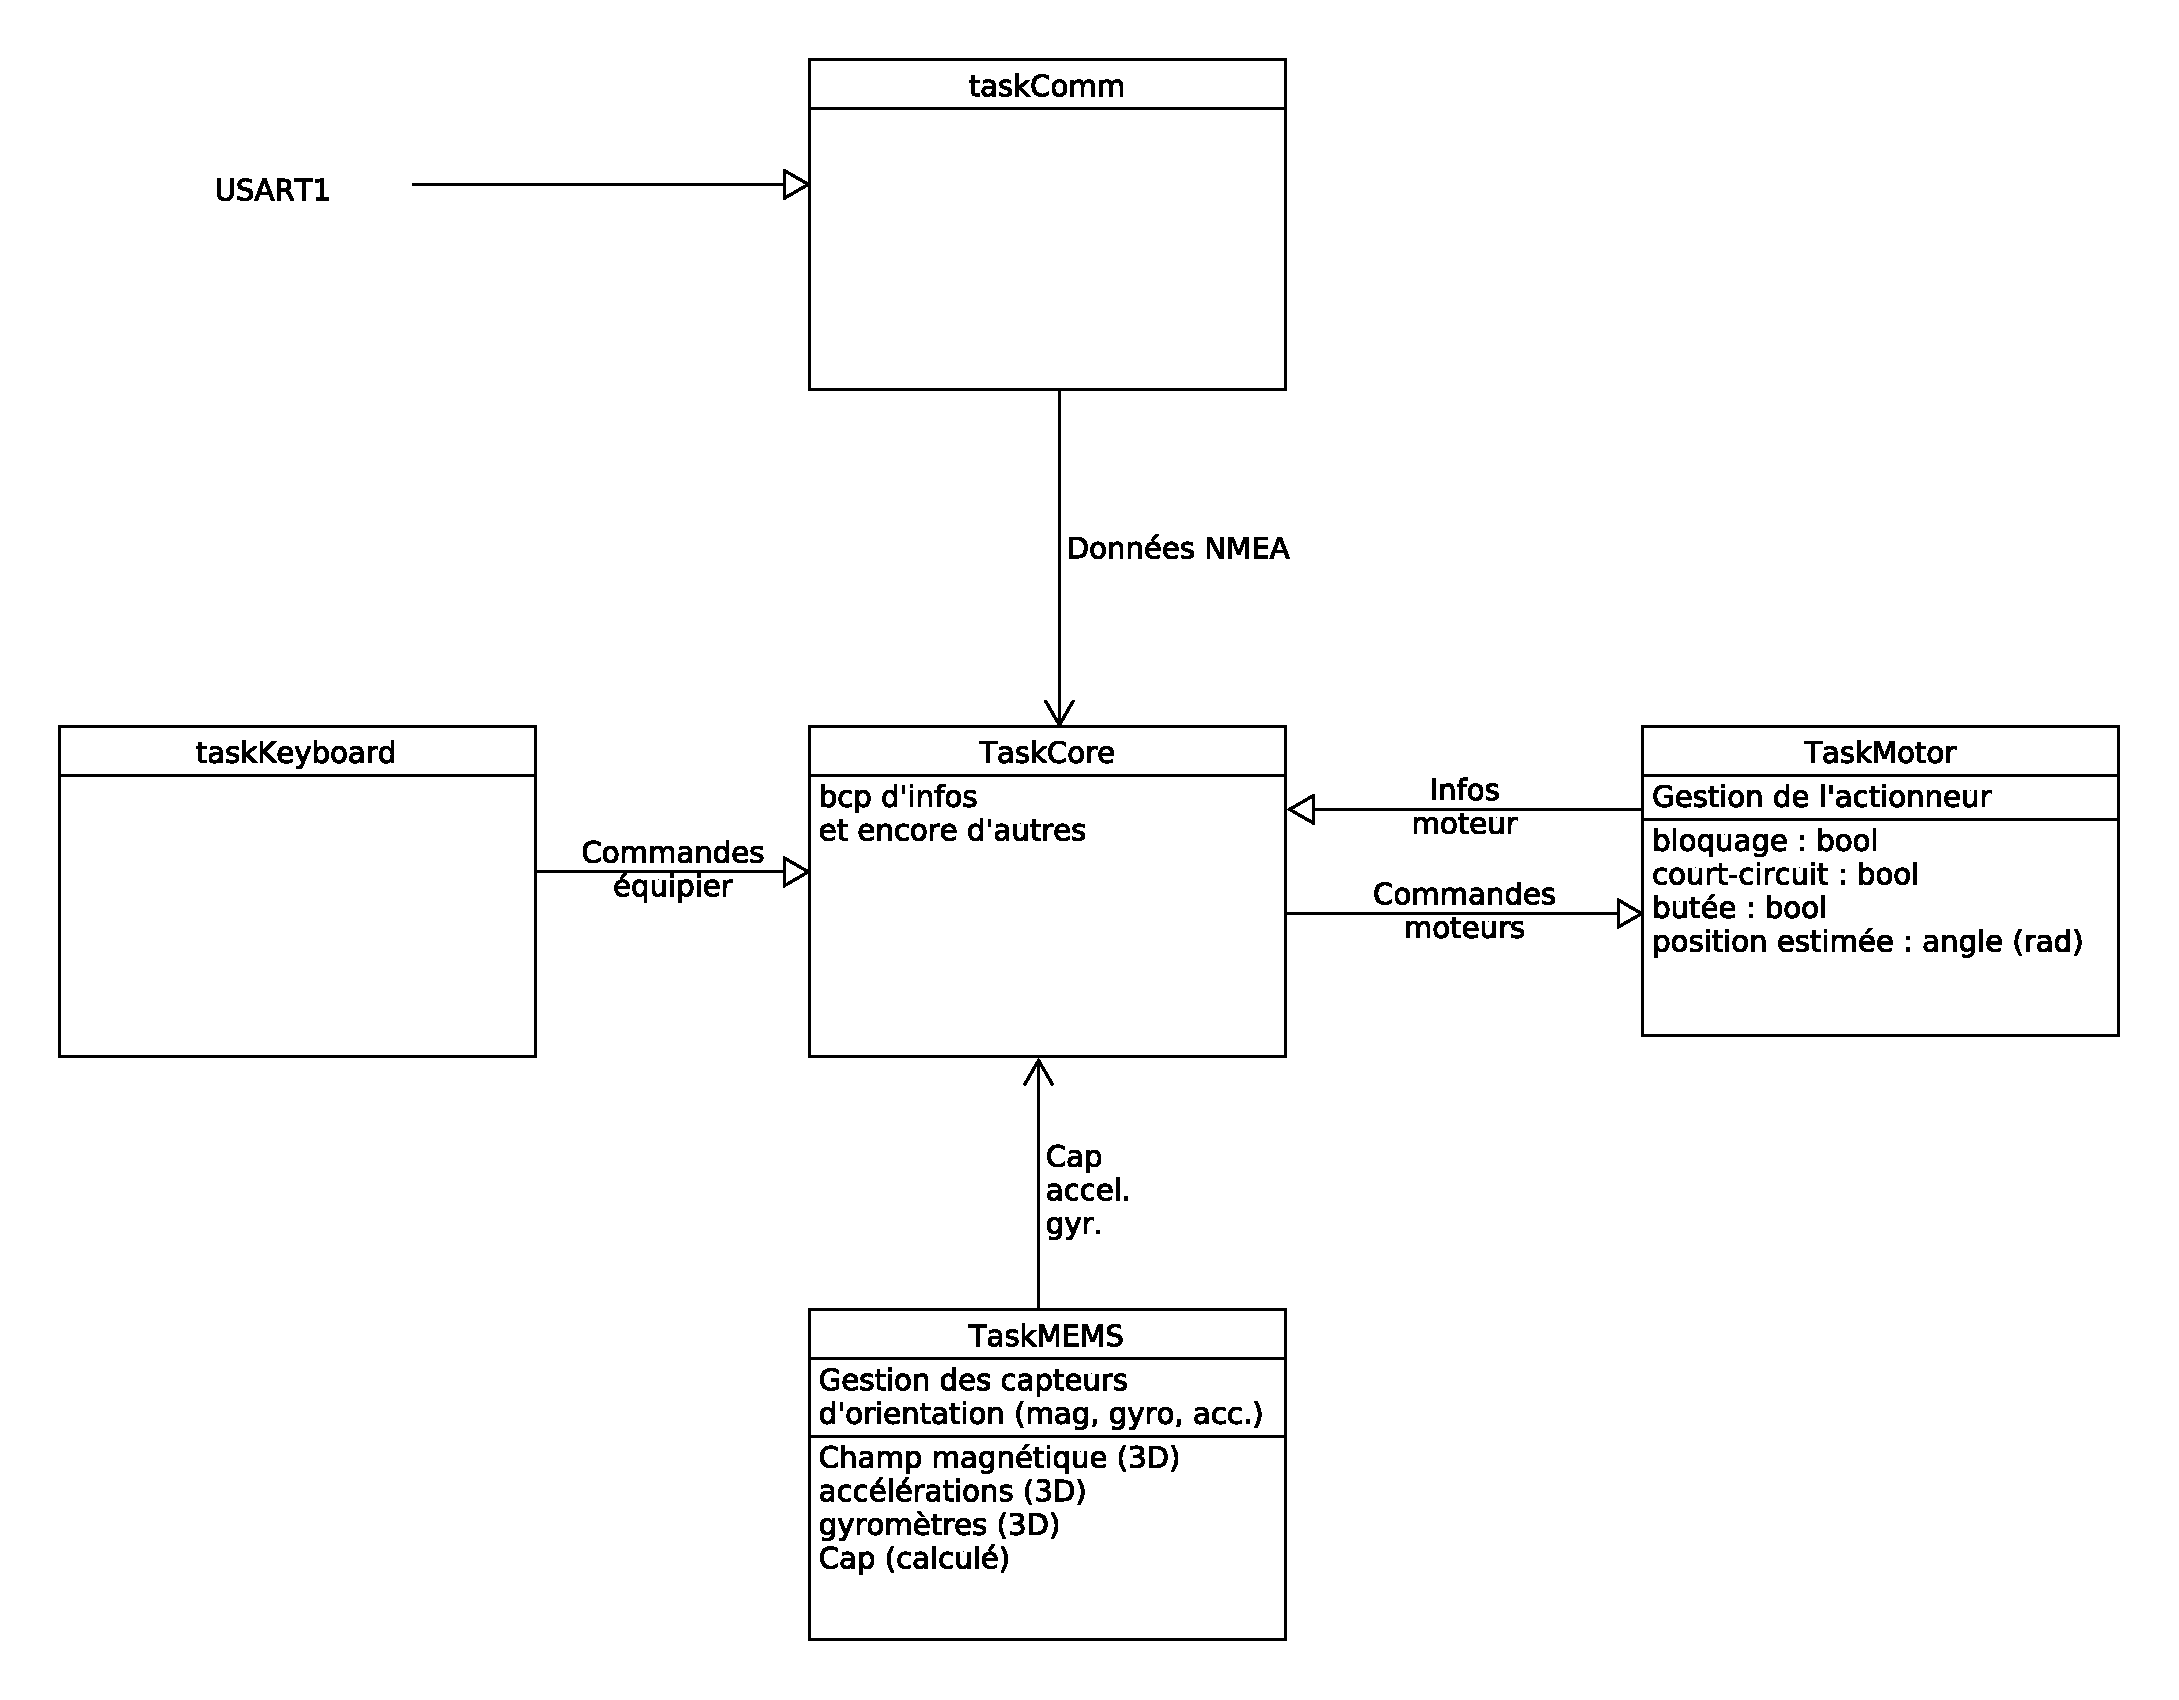
\includegraphics[scale=0.3]{diagram-Taches}
	\caption{Flots de données entre les tâches}
\end{figure}

\subsection{ScrutationClavier}
La tâche utilise la fonction nommée TaskKeyboard qui n'utilise aucun argument.
Elle fonctionne par scrutation périodique des entrées sur lesquelles sont branchées les touches.
La scrutation périodique est utilisée car les touches provoquaient de très nombreux
rebonds parasites. 
Elle envoie les ordres à la tâche de gestion de l'état
par l'intermédiaire d'un \texttt{MessageBuffer\_t} nommé buffclav.

\subsection{Contrôle du moteur}
Cette tâche reçoit les ordres de la tâche de gestion,
elle commande l'embrayage du moteur et son fonctionnement : sens et durée.
Elle corrige la durée de fonctionnement en fonction de l'effort du moteur.
Lorsque le moteur tourne, elle mesure le courant du moteur,
vérifie que le moteur n'est pas bloqué ou débranché et
renvoie une estimation de l'effort du moteur. Elle informe la tâche principale
lorsque le moteur a fini un mouvement demandé.
\subsubsection{Entrées}

\begin{itemize}
  \item Ordres de commande du moteur et de l'embrayage en provenance de la tâche principale;
  \item valeurs du courant et de la tension en provenance de l'ADC;
  \item horloge (à définir).
\end{itemize}
\subsubsection{Sorties}
\begin{itemize}
	\item ordres vers le moteur mise en marche et sens;
	\item ordres vers l'embrayage : enclenchement et désenclenchement ;
	\item informations vers la tâche principale sur le fonctionnement du moteur estimation de l'effort, de la position, blocage ou court-circuit.
\end{itemize}
\subsection{Gestion des capteurs MEMS}
Cette tâche lit les informations des capteurs MEMs, les filtre,
calcule le cap et le lacet et envoie les informations traitées à la tâche principale.
Les documents de ré



Le signal d'interruption n'étant pas disponible sur la carte de Pololu
la tâche fonctionne par scrutation.

\subsubsection{Sorties}
La tâche envoie les données vers la tâche principale.
\subsection{Tâche principale}
\subsubsection{Entrées}
\begin{itemize}
  \item Commandes en provenance du clavier;
  \item Informations du moteur;
  \item Informations des capteurs MEMS ;
  \item Informations en provenance des interfaces NMEA
  \item horloge (à définir).
\end{itemize}
\subsubsection{Sorties}
\begin{itemize}
  \item Commandes moteurs;
  \item alarmes;
\end{itemize}

\section{Canaux de communications}

\begin{tabular}{|l|c|c|c|}
\hline
Canal & Nom & Type & Taille \\
\hline
Messages vers le gestionnaire principal & \texttt{bufferCore} & \texttt{MessageBuffer\_t} & 10 \\
\hline 
Ordres vers le moteur & \texttt{bufferMotor} & \texttt{MessageBuffer\_t} & 5 \\ 
\hline
\end{tabular}
\subsection{Message gestionnaire principal}
Ces messages sont envoyés par les tâches TaskKeyboard, TaskMotor et TaskMEMs.
Il sont stockés dans une structure dont les deux premiers octets comportent
un code indiquant la nature du message et, en option, d'autres informations.
\\
\begin{tabular}{|l|l|}
\hline 
Ordre & Code et valeurs optionnelles \\
\hline
\multicolumn{2}{|c|}{Ordres en provenance de la tâche du clavier vers la tâche principale} \\
\hline 
Mise en mode automatique & MSG\_KBD\_AUTO \\ 
Mise en veille & MSG\_KBD\_STDBY \\ 
+1 & MSG\_KBD\_STARBOARD\_ONE \\ 
-1 & MSG\_KBD\_PORT\_ONE \\ 
+10 & MSG\_KBD\_STARBOARD\_TEN \\ 
-10 & MSG\_KBD\_PORT\_TEN \\ 
+1 relachée & MSG\_KBD\_STARBOARD\_ONE\_END \\ 
-1 relachée & MSG\_KBD\_PORT\_ONE\_END \\ 
\hline 
\multicolumn{2}{|c|}{Informations en provenance de la tâche de gestion du moteur} \\
\hline
Position estimée du moteur & MSG\_MOT\_POSITION\_ESTIMEE \\
Effort moteur & MSG\_MOT\_EFFORT + float effort\\ 
Moteur bloqué ou en butée & MSG\_MOT\_BLOCKED \\
Court-circuit sortie moteur & MSG\_MOT\_SHORT\_CIRCUIT \\
Fin de déplacement actuateur & MSG\_MOT\_END\_MOVE + float : effort \\
\hline
\multicolumn{2}{|c|}{Informations des capteurs MEMs}\\
\hline
Info Capteurs MEMs & MSG\_MEMS\_VALUES + 2 floats : cap et lacet \\
Info MEMs indisponible & MSG\_MEMS\_FAILURE \\

\hline
\end{tabular} 
\subsection{Commandes envoyées à la tâche de gestion du moteur}
Ces messages sont envoyés par la tâche principale ou un timer
à la tâche de gestion du moteur.
\\
\begin{tabular}{|l|l|}
	\hline 
	Ordre & Code et valeurs optionnelles \\ 
	\hline
	\multicolumn{2}{|c|}{Commande de la tâche principale} \\
	\hline 
    Enclenchement de l'embrayage & MSG\_MOT\_EMBRAYE\\
    Désenclenchement de l'embrayage & MSG\_MOT\_DEBRAYE\\
    Mise en marche vers tribord & MSG\_MOT\_STARBOARD\\
    Mise en marche vers babord  & MSG\_MOT\_PORT\\
    Mouvement vers tribord & MSG\_MOT\_MOVE\_STARBOARD + float : valeur\\
    Mouvement vers babord  & MSG\_MOT\_MOVE\_PORT + float: valeur\\
    Arrêt du moteur & MSG\_MOT\_STOP\\
    Demande de mesure d'effort & MSG\_MOT\_DMD\_EFFORT\\
    \hline
	\multicolumn{2}{|c|}{commande du timer} \\
	\hline
	Commande du TIMER & MSG\_MOT\_MOVING\_CONTROL\\
    \hline
\end{tabular} 

La tâche de gestion du moteur effectue les déplacements
dont l'amplitude doit être proportionnelle à la valeur en paramètre,
elle adapte la durée au courant du moteur.


\end{document}

